\documentclass{libs/XJTLU_format}
% Inserting the preamble file with the packages
%%%%%%%%%%%%%%%%%%%%%%%%%%%%%%%%%%%%%%%%%%%%%%%%%%%%%%%%%%%%%%%%%%%%%
%% This file contains the packages that can be used in the beamer. %%
%%%%%%%%%%%%%%%%%%%%%%%%%%%%%%%%%%%%%%%%%%%%%%%%%%%%%%%%%%%%%%%%%%%%%
% Package to fonts family
\usepackage[T1]{fontenc}
% Package to accentuation
\usepackage[utf8]{inputenc}
% Package to Figures
\usepackage{graphicx}
% Package to the colors
\usepackage{color}
% Package to the colors
\usepackage{xcolor}
% Packages to math symbols and expressions
\usepackage{amsfonts, amssymb, amsmath}
% Package to multiple lines and columns in table
\usepackage{multirow, array} 
% Package to create pseudo-code
% For more detail of this package: http://linorg.usp.br/CTAN/macros/latex/contrib/algorithm2e/doc/algorithm2e.pdf
\usepackage{algorithm2e}
% Package to insert code
\usepackage{listings} 
\usepackage{keyval}
% Package to justify text
\usepackage[document]{ragged2e}
% Package to manage the bibliography
\usepackage[backend=biber, style=numeric, sorting=none]{biblatex}
% Package to facilities quotations
\usepackage{csquotes}
% Package to use multicols
\usepackage{multicol}
\usepackage{transparent}

% Inserting the references file

\usepackage [spanish]{babel}
\usepackage [utf 8]{inputenc}

% Title
\title[Curso Análisis exploratorio de datos en Python y R]{\huge\textbf{Curso Análisis exploratorio de datos en Python y R}}
% Subtitle
\subtitle{Introducción y objetivos}
% Author of the presentation
\author{Juan Camilo Perdomo}
% Institute's Name
\institute[Universidad del Rosario]{
    % email for contact
    \normalsize{\email{juan.perdomor@urosario.edu.co}}
    \newline
    % University name
    \university{Universidad del Rosario}
    \newline
    % Department Name
    \department{Bogotá, Colombia}
}
% date of the presentation
\date{\today}

%%%%%%%%%%%%%%%%%%%%%%%%%%%%%%%%%%%%%%%%%%%%%%%%%%%%%%%%%%%%%%%%%%%%%%%%%%%%%%%%%%
\begin{document}
% insert the code style
%%%%%%%%%%%%%%%%%%%%%%%%%%%%%%%%%%%%%%%%%%%%%%%%%%%%%%%%%%%%%%%%%%%%%%%%%%%%%%%%%%%
%% This file contains the style of the codes show in slides.                     %%
%% The package used is listings, but it possible to used others.                 %%
%%%%%%%%%%%%%%%%%%%%%%%%%%%%%%%%%%%%%%%%%%%%%%%%%%%%%%%%%%%%%%%%%%%%%%%%%%%%%%%%%%%

% color used in the code style
\definecolor{codegreen}{rgb}{0,0.6,0}
\definecolor{codegray}{rgb}{0.5,0.5,0.5}
\definecolor{codepurple}{rgb}{0.58,0,0.82}
\definecolor{codebackground}{rgb}{0.95,0.95,0.92}

% style of the code!
\lstdefinestyle{codestyle}{
    backgroundcolor=\color{codebackground},   
    commentstyle=\color{codegreen},
    keywordstyle=\color{magenta},
    numberstyle=\tiny\color{codegray},
    stringstyle=\color{codepurple},
    basicstyle=\ttfamily\footnotesize,
    frame=single,
    breakatwhitespace=false,         
    breaklines=true,                 
    captionpos=b,                    
    keepspaces=true,                 
    numbers=left,                    
    numbersep=5pt,                  
    showspaces=false,                
    showstringspaces=false,
    showtabs=false,                  
    tabsize=2,
    title=\lstname 
}

\lstset{style=codestyle}



%% ---------------------------------------------------------------------------
% First frame (with tile, subtitle, ...)
\begin{frame}{}
    \maketitle
\end{frame}

%% ---------------------------------------------------------------------------
% Second frame
\begin{frame}{Tabla de contenidos}
    \tableofcontents
\end{frame}

%% ---------------------------------------------------------------------------
\section{¿Qué es el análisis exploratorio de datos?}

\begin{frame}[fragile] 
    \frametitle{Análisis exploratorio de datos}
    \begin{center}
        El Análisis Exploratorio de Datos, conocido por sus siglas en inglés EDA (Exploratory Data Analysis), es considerado como el conjunto de procedimientos cuyo objetivo general es proporcionar una visión más detallada y precisa de la información (variables, indicadores, índices, entre otros) almacenada en un dataset, previo al uso de técnicas estadísticas inferenciales. \newline
    \end{center}

    \begin{center}
        Se apoya en un planteamiento descriptivo y se realiza  con una mentalidad “exploratoria”. Desde un punto de vista técnico, el EDA se caracteriza por el empleo de procedimientos analíticos y descriptivos de carácter gráfico o semigráfico, que muestren todas las particularidades y carácteres de las variables sacando a la luz las estructuras ocultas de los datos.(Rodríguez Jaume y Mora, 2001).
    \end{center}
\end{frame}

%% ---------------------------------------------------------------------------

\begin{frame}[fragile] 
    \frametitle{Análisis exploratorio de datos, una vista gráfica}
    
 De acuerdo con el portal "Towards Data Science", el análisis de datos luce de la siguiente manera: \newline
 
     \begin{figure}[H]
        \centering
            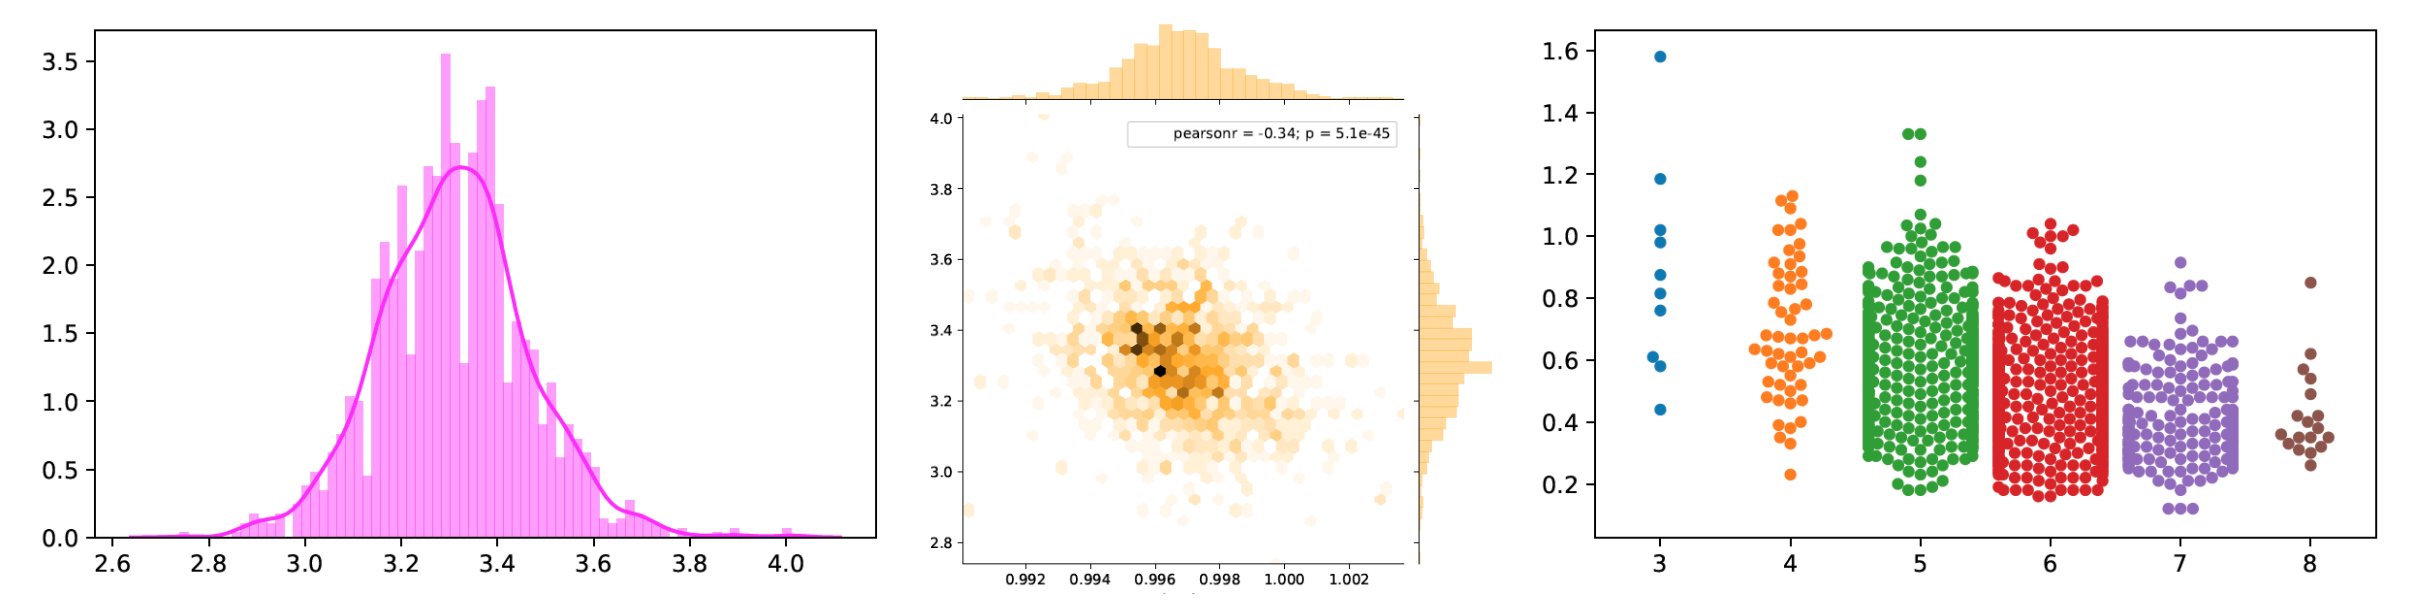
\includegraphics [width =1.0\textwidth]{Graphs.png}
        \caption{Tipos de gráficos para el EDA (Towards Data Science, 2018)}
    \end{figure}

\end{frame}

%% --------------------------------------------------------------------------

\begin{frame}[fragile] 
    \frametitle{Análisis exploratorio de datos}
    \begin{center}
        En otras palabras, el análisis exploratorio de datos es un primer encuentro con los datos, donde se explora el número de estos, unidades de análisis, periodicidades, distribuciones, relaciones entre variables e información que va mucho más allá.  Esto es posible hacerlo de una manera "manual", a través de Excel; sin embargo, existen softwares que permiten automatizar estos procesos y desarrollarlos de una manera más confiable y sencilla.\newline 
    \end{center}
    
    \begin{center}    
        Además, es posible hacer uso de la estadística descriptiva (en el curso se verá la diferencia con la estadística inferencial) para conocer mejor nuestros datos: medidas de tendencia central, de dispersión y sus distribuciones. 
    \end{center}

\end{frame}

%% ---------------------------------------------------------------------------
\section{Software estadístico para el análisis de datos}

\begin{frame}[fragile] 
    \frametitle{Software estadístico para el análisis de datos} 
Existen diversos programas,aplicaciones, paquetes, softwares e, incluso, lenguajes de programación que permiten realizar exploración, análisis, cálculos, inferencia, ilustración, entre otros, de los datos.\newline   

--------------------------------------------------------------------------------------------\newline  


\begin{multicols}{3}
    \begin{figure}[H]
        \raggedright
            
\includegraphics [width =0.2\textwidth]{excel-logo.jpeg}
    \end{figure}
    \begin{figure}[H]
            
\includegraphics [width =0.2\textwidth]{images.png}
    \end{figure}
        \begin{figure}[H]
            
\includegraphics [width =0.2\textwidth]{spss-herramienta-de-analisis-estadistico.jpeg}\newline
    \end{figure} 
        \begin{figure}[H]
        \raggedright
            
\includegraphics [width =0.22\textwidth]{python.png}
    \end{figure}
    \begin{figure}[H]
            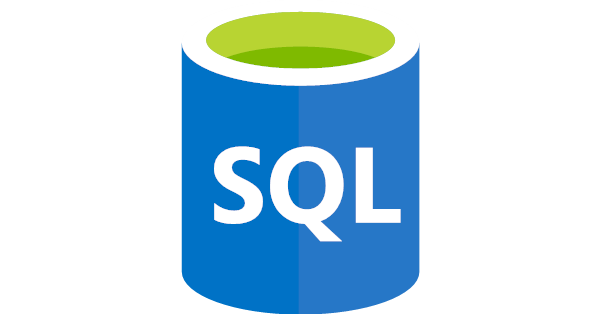
\includegraphics [width =0.2\textwidth]{sql.png}
    \end{figure}
        \begin{figure}[H]
            
\includegraphics [width =0.13\textwidth]{r.png}
    \end{figure}
\end{multicols}
--------------------------------------------------------------------------------------------
\end{frame}

%% ---------------------------------------------------------------------------

\begin{frame}[fragile] 
    \frametitle{Software estadístico para el análisis de datos}

    \begin{center}
Este curso estará basado en los dos últimos (Python y R), dado que son de uso libre (gratuito) y, además, porque son los dos que están tomando, no solo mayor popularidad e importancia, sino que son las que más han crecido en los últimos años en términos de paquetes y librerías en el mundo del análisis y, en general, de la ciencia de datos.\newline    
    \end{center}

\begin{multicols}{2}
    \begin{figure}[H]
            
\includegraphics [width =0.4\textwidth]{python.png}
    \end{figure}
        \begin{figure}[H]
            
\includegraphics [width =0.25\textwidth]{r.png}
    \end{figure}
\end{multicols}
\end{frame}

%% ---------------------------------------------------------------------------
\section{¿Qué es Python?}

\begin{frame}[fragile] 
    \frametitle{Python / Jupyter Notebook}

    \begin{center}
De acuerdo con el portal de Crehana, Python es un lenguaje de programación interpretado, multiparadigma y multiplataforma usado, principalmente, en Big Data, AI (Inteligencia Artificial), Data Science, frameworks de pruebas y desarrollo web. Esto lo convierte en un lenguaje de propósito general de gran nivel debido a su extensa biblioteca, cuya colección ofrece una amplia gama de instalaciones.\newline    
    \end{center}

\begin{multicols}{2}
    \begin{center}
    {\color{yellow}{\small Su uso se da principalmente en una herramienta llamada Jupyter Notebook, cuya funcionalidad es interpretar el código en lenguaje Python (iPython) y mostrar sus resultados a pie de línea de una manera interactiva.}}
    \end{center}
    
    \begin{figure}[H]
            
\includegraphics [width =0.61\textwidth]{Jupyter.png}
    \end{figure}
\end{multicols}
\end{frame}

%% ---------------------------------------------------------------------------
\section{¿Qué es R?}

\begin{frame}[fragile] 
    \frametitle{R / R-Studio}

    \begin{center}
De acuerdo con su propio portal, R es un entorno de software libre para gráficos y computación estadística. Se compila y se ejecuta en una amplia variedad de plataformas UNIX, Windows y MacOS, es también un lenguaje de programación, utilizado principalmente en la ciencia de datos y el análisis de datos.\newline    
    \end{center}

\begin{multicols}{2}
    \begin{center}
    {\color{aqua}{\small Tal como en Python, R tiene un intérprete (R-Studio) que permite programar en este lenguaje y mostrar sus resultados en una interfaz de manera interactiva. Aunque, R también está siendo usado en otros sofware para edición de texto, como Visual Studio Code.}}
    \end{center}
    
    \begin{figure}[H]
            
\includegraphics [width =0.51\textwidth]{RStuido.png}
    \end{figure}
\end{multicols}
\end{frame}

%% ---------------------------------------------------------------------------

\section{Bibliografía}
\begin{frame}{Bibliografía}
    % Beamer does not support BibTeX so references must be inserted manually as below
    \footnotesize{
        \begin{thebibliography}{p1}
            \bibitem[Rodríguez Jaume y Mora, 2001]{p1} Rodríguez-Jaume, María-José y Mora Catalá, Rafael (2001)
            \newblock {Análisis de regresión múltiple}
            \newblock {Universidad de Alicante, Departamento de Sociología}.\newblock {http://rua.ua.es/dspace/handle/10045/8143}\newline
        \end{thebibliography}
        
        \begin{thebibliography}{p1}
            \bibitem[Towards Data Science, 2018]{p1} Towards Data Science (2018)
            \newblock {What is Exploratory Data Analysis?}
            \newblock {https://towardsdatascience.com/exploratory-data-analysis-8fc1cb20fd15}\newline
        \end{thebibliography}
        
            \begin{thebibliography}{p1}
            \bibitem[Crehana, 2021]{p1} Crehana (2021)
            \newblock {¿Qué es Python? El lenguaje de programación más popular para aprender en 2021}
            \newblock {https://www.crehana.com/co/blog/web/que-es-python/}\newline
        \end{thebibliography}
        
            \begin{thebibliography}{p1}
            \bibitem[r-project Org, 2021]{p1} r-project Org (2021)
            \newblock {The R Project for Statistical Computing}
            \newblock {https://www.r-project.org/}\newline
        \end{thebibliography}
    }
\end{frame}

%% ---------------------------------------------------------------------------
\end{document}